\subsection{\IFRU{Работа с битовыми полями в структуре}{Bit fields in structure}}

\subsubsection{\IFRU{Пример CPUID}{CPUID example}}

\IFRU{Язык \CCpp позволяет укзывать, сколько именно бит отвести для каждого поля структуры. 
Это удобно если нужно экономить место в памяти. К примеру, для переменной типа \Tbool достаточно одного бита.
Но, это не очень удобно, если нужна скорость.}
{\CCpp language allow to define exact number of bits for each structure fields.
It is very useful if one needs to save memory space. 
For example, one bit is enough for variable of \Tbool type.
But of course, it is not rational if speed is important.}

\newcommand{\FNCPUID}{\footnote{\url{http://en.wikipedia.org/wiki/CPUID}}}

\index{x86!\Instructions!CPUID}
\IFRU{Рассмотрим пример с инструкцией \CPUID\FNCPUID. 
Эта инструкция возвращает информацию о том, какой процессор имеется в наличии и какие фичи он имеет.}
{Let's consider \CPUID\FNCPUID instruction example.
This instruction returning information about current CPU and its features.}

\IFRU{Если перед исполнением инструкции в \EAX будет 1, 
то \CPUID вернет упакованную в \EAX такую информацию о процессоре:}
{If the \EAX is set to 1 before instruction execution, 
\CPUID will return this information packed into the \EAX register:}

\begin{center}
\begin{tabular}{ | l | l | }
\hline
3:0 & Stepping \\
7:4 & Model \\
11:8 & Family \\
13:12 & Processor Type \\
19:16 & Extended Model \\
27:20 & Extended Family \\
\hline
\end{tabular}
\end{center}

\newcommand{\FNGCCAS}{\footnote{\href{http://www.ibiblio.org/gferg/ldp/GCC-Inline-Assembly-HOWTO.html}
{\IFRU{Подробнее о встроенном ассемблере GCC}{More about internal GCC assembler}}}}

\IFRU{MSVC 2010 имеет макрос для \CPUID, а GCC 4.4.1 ~--- нет. 
Поэтому для GCC сделаем эту функцию сами, используя его встроенный ассемблер\FNGCCAS.}
{MSVC 2010 has \CPUID macro, but GCC 4.4.1 ~--- has not.
So let's make this function by yourself for GCC with the help of its built-in assembler\FNGCCAS.}

\lstinputlisting{15_structs/CPUID.c}

\IFRU{После того как \CPUID заполнит \EAX/\EBX/\ECX/\EDX, у нас они отразятся в массиве \TT{b[]}. 
Затем, мы имеем указатель на структуру \TT{CPUID\_1\_EAX}, и мы указываем его на значение 
\EAX из массива \TT{b[]}.}
{After \CPUID will fill \EAX/\EBX/\ECX/\EDX, these registers will be reflected in the \TT{b[]} array.
Then, we have a pointer to the \TT{CPUID\_1\_EAX} structure and we point it to the value in the \EAX from \TT{b[]} array.}

\IFRU{Иными словами, мы трактуем 32-битный \Tint как структуру.}
{In other words, we treat 32-bit \Tint value as a structure.}

\IFRU{Затем мы читаем из структуры.}{Then we read from the stucture.}

\IFRU{Компилируем в MSVC 2008 с опцией \Ox}{Let's compile it in MSVC 2008 with \Ox option}:

\lstinputlisting[caption=\Optimizing MSVC 2008]{15_structs/CPUID_msvc_Ox.asm}

\index{x86!\Instructions!SHR}
\IFRU{Инструкция \TT{SHR} сдвигает значение из \EAX на то количество бит, 
которое нужно \IT{пропустить}, то есть, мы игнорируем некоторые биты \IT{справа}.}
{\TT{SHR} instruction shifting value in the \EAX register by number of bits should be
\IT{skipped}, e.g., we ignore some bits \IT{at right}.}

\index{x86!\Instructions!AND}
\IFRU{А инструкция \ANDIns очищает биты \IT{слева} которые нам не нужны, или же, говоря иначе, 
она оставляет по маске только те биты в \EAX, которые нам сейчас нужны.}
{\ANDIns instruction clears bits not needed \IT{at left}, or, in other words, 
leaves only those bits in the \EAX register we need now.}

\IFRU{Попробуем GCC 4.4.1 с опцией \Othree.}{Let's try GCC 4.4.1 with \Othree option.}

\lstinputlisting[caption=\Optimizing GCC 4.4.1]{15_structs/CPUID_gcc_O3.asm}

\IFRU{Практически, то же самое. Единственное что стоит отметить это то, что GCC решил зачем-то объеденить 
вычисление \TT{extended\_model\_id} и \TT{extended\_family\_id} в один блок, 
вместо того чтобы вычислять их перед соответствующим вызовом \printf.}
{Almost the same. The only thing worth noting is that GCC somehow united calculation of
\TT{extended\_model\_id} and \TT{extended\_family\_id} into one block,
instead of calculating them separately, before corresponding each \printf call.}

\subsubsection{\WorkingWithFloatAsWithStructSubSubSectionName}
\label{sec:floatasstruct}

\IFRU{Как уже раннее указывалось в секции о FPU~\ref{sec:FPU}, и \Tfloat и \Tdouble содержат в себе знак, 
мантиссу и экспоненту. 
Однако, можем ли мы работать с этими полями напрямую? Попробуем с \Tfloat.}
{As it was already noted in section about FPU~\ref{sec:FPU}, both \Tfloat and \Tdouble types consisted of sign,
significand (or fraction) and exponent.
But will we able to work with these fields directly? Let's try with \Tfloat.}

\index{IEEE 754}
\index{float}
\begin{figure}[ht!]
\centering
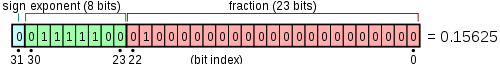
\includegraphics[scale=0.66]{15_structs/500px-Float_example.png}
\caption{\IFRU{Формат значения float\protect\footnotemark}
{float value format\protect\footnotemark}}
\end{figure}

\footnotetext{\IFRU{иллюстрация взята из}{illustration taken from} wikipedia}

\lstinputlisting{15_structs/float_en.c}

\IFRU{Структура \TT{float\_as\_struct} занимает в памяти столько же места сколько и \Tfloat, 
то есть 4 байта или 32 бита.}
{\TT{float\_as\_struct} structure occupies as much space is memory as \Tfloat, e.g., 4 bytes or 32 bits.}

\IFRU{Далее мы выставляем во входящем значении отрицательный знак, 
а также прибавляя двойку к экспоненте, мы тем 
самым умножаем всё значение на \TT{$2^2$}, то есть на 4.}
{Now we setting negative sign in input value and also by addding 2 to exponent we thereby multiplicating
the whole number by \TT{$2^2$}, e.g., by 4.}

\IFRU{Компилируем в MSVC 2008 без оптимизации:}{Let's compile in MSVC 2008 without optimization:}

\lstinputlisting[caption=\NonOptimizing MSVC 2008]
{\IFRU{15_structs/float_msvc_ru.asm}{15_structs/float_msvc_en.asm}}

\IFRU{Слекга избыточно. В версии скомпилированной с флагом \Ox нет вызовов \TT{memcpy()}, 
там работа происходит сразу с переменной f. Но по неоптимизированной версии будет проще понять.}
{Redundant for a bit. If it compiled with \Ox flag there are no \TT{memcpy()} call,
f variable is used directly. But it is easier to understand it all considering unoptimized version.}

\IFRU{А что сделает GCC 4.4.1 с опцией \TT{-O3}?}{What GCC 4.4.1 with \TT{-O3} will do?}

\lstinputlisting[caption=\Optimizing GCC 4.4.1]
{\IFRU{15_structs/float_gcc_O3_ru.asm}{15_structs/float_gcc_O3_en.asm}}

\IFRU{Да, функция \TT{f()} в целом понятна. Однако, что интересно, еще при компиляции, 
не взирая на мешанину с полями структуры, GCC умудрился вычислить результат функции \TT{f(1.234)} и 
сразу подставить его в аргумент для \printf{}!}
{The \TT{f()} function is almost understandable. However, what is interesting, GCC was able to calculate
\TT{f(1.234)} result during compilation stage despite all this hodge-podge with structure fields
and prepared this argument to the \printf{} as precalculated!}


